\section{Experiments}~\label{experiment}
We evaluate our method in simulation and on physical robots. The evaluation covers WasteSorting and TomatoHarvesting. We first compare the complete query policies in simulation with correct oracle responses. We then evaluate physical robot execution with responses from a vision-language model (VLM) and human participants. Ablation experiments examine the contributions of query timing and query selection. A threshold sweep examines the balance between task success and query count.

The oracle experiments include $200$ trials per domain and condition. The VLM experiments include $40$ trials per domain and method. The planned human evaluation is designed for five participants with $10$ trials per domain and method for a total of $40$ trials.

\begin{figure}[t!]
    %\captionsetup{skip=0pt} % \hspace{0.3cm}
    \begin{center}
  
    \begin{subfigure}[b]{0.47\textwidth}
        \captionsetup{skip=0pt}
	    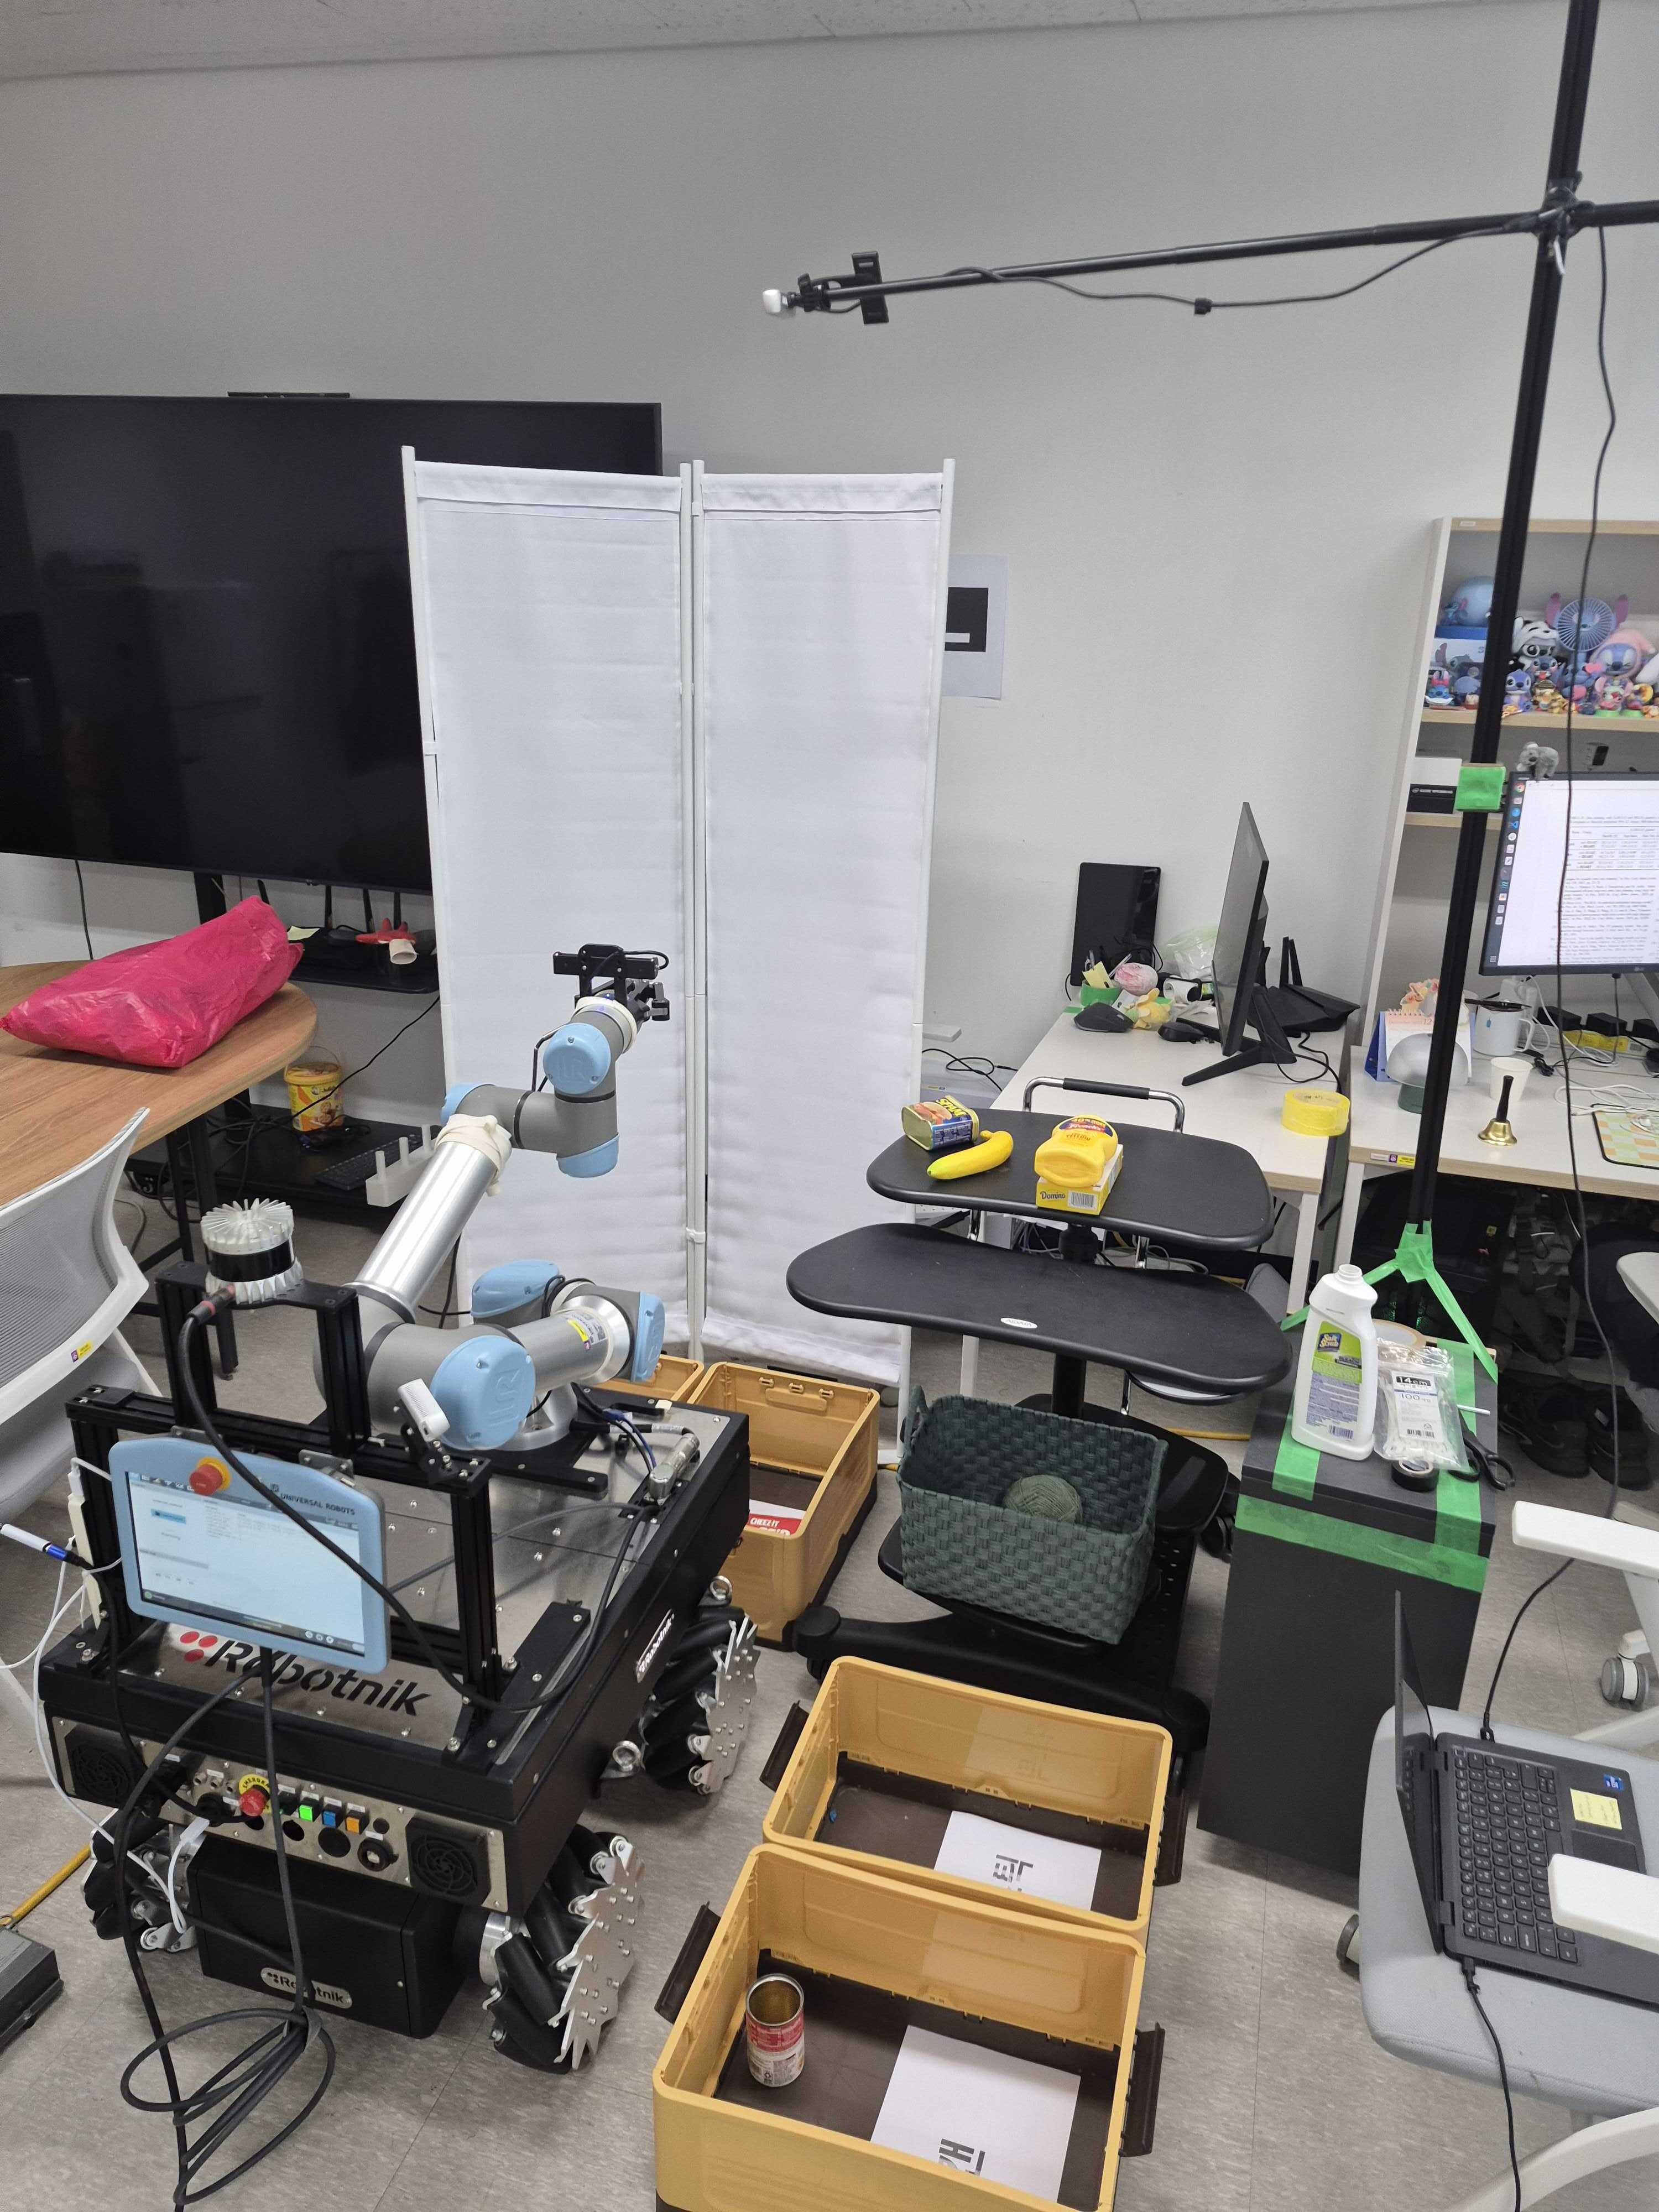
\includegraphics[width=\textwidth]{figures/WasteSortingEnv.jpg}
        \caption{WasteSorting domain.}
        \label{fig:dom1}
    \end{subfigure}
    \quad
    \begin{subfigure}[b]{0.47\textwidth}
        \captionsetup{skip=0pt}
	    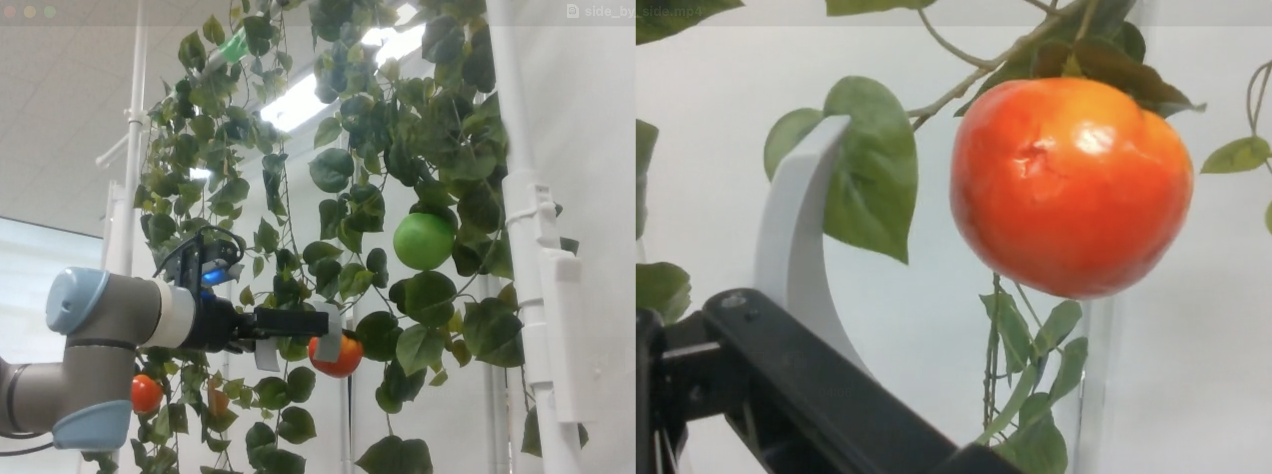
\includegraphics[width=\textwidth]{figures/fig_exp_setup2.pdf}
	    \caption{TomatoHarvesting domain.}
        \label{fig:dom2}
    \end{subfigure}
    \caption{Physical robot environments. (a) A fixed UR5e robot sorts objects from four waste categories into designated bins in a tabletop workspace. (b) A mobile manipulator harvests ripe tomatoes and discards rotten tomatoes.}
  \label{fig:env_setting}
  
  \end{center}
\end{figure}


\subsection{Experimental Setup}~\label{exp:setup}
The oracle experiments use simulated task execution and exact external responses. The VLM and human experiments use physical robots in laboratory environments. Figure~\ref{fig:env_setting} shows the physical setups. \textbf{WasteSorting} uses a fixed UR5e robot arm. \textbf{TomatoHarvesting} uses a Summit mobile platform equipped with a UR5e robot arm. The mobile platform uses an RGB-D camera for perception and LiDAR for localization. WasteSorting uses SAM3 for object detection~\cite{carion2025sam3segmentconcepts}. TomatoHarvesting uses YOLOv12 for object detection~\cite{tian2025yolov12}.


\subsubsection{Task Domains}~\label{exp:setup_domains}
The WasteSorting task requires the robot to place every object in the correct bin. The UR5e robot is positioned between the objects and recycling bins in Fig.~\ref{fig:dom1}. All objects are within reach. The robot can detect objects and then pick and place them. Each object belongs to one of four waste categories corresponding to general waste or recyclable paper or cans or plastic. The categories are initially unknown. The main sources of uncertainty in this domain are occlusion and noisy sensor observations. In simulation we randomize the initial object arrangement for each trial. A trial succeeds if the robot places all objects in the correct bins within the step limit. Each correct placement yields a task reward of $+5$. Completion of the task yields an additional reward of $+10$. A penalty of $-10$ applies to the third and each subsequent detection action in a consecutive sequence.

The TomatoHarvesting task requires the robot to harvest fresh ripe tomatoes and discard rotten tomatoes. Four tomatoes are distributed across two stems in Fig.~\ref{fig:dom2}. The robot navigates between the docking station and the two stems. The \texttt{detect} action distinguishes ripe from unripe tomatoes. After a tomato is picked the \texttt{scan} action distinguishes fresh from rotten tomatoes. The robot uses \texttt{place} for fresh tomatoes and \texttt{discard} for rotten tomatoes. Unripe tomatoes remain on the stem. The main source of uncertainty in this domain is noisy sensor observations. In simulation we randomize tomato locations across the two stems for each trial. A trial succeeds if all fresh ripe tomatoes are harvested and all rotten tomatoes are discarded within the step limit. Correct placement of a fresh tomato or disposal of a rotten tomato yields a task reward of $+10$. Consecutive \texttt{detect} actions at the same stem and consecutive \texttt{scan} actions on the same tomato incur a penalty of $-5$ from the second action onward.


\subsubsection{Implementation Details}~\label{exp:details}
Our POMCP planner uses $100$ simulations per planning step with a maximum simulation depth of $20$. The discount factor is $\gamma=0.2$ and the UCB exploration constant is $c=1.0$. The default confidence threshold is $\tau=0.8$. We use Gemma 4 31B IT with NVFP4 quantization~\cite{gemmateam2026gemma4} as the external expert in the VLM experiments. Appendix~\ref{appx:settings} provides the baseline configurations and additional experimental details.

\subsubsection{Evaluation Metrics}~\label{exp:metrics}
Success rate is the fraction of all trials that achieve the task goal within the trial limit. Query count is the number of external requests per trial. Query probability is the fraction of physical steps that trigger at least one query. Plan length is the number of physical actions executed per trial. Search time is the cumulative time spent on plan search per trial. Interaction time is the cumulative time spent on external requests and response processing per trial. We report interaction time only for the VLM and human experiments. We note that all metrics except success rate use successful trials.
